% -*- latex -*-

\chapter{Basic Usage}
\label{chap:Basic_Usage}

In this chapter we describe in greater detail the basic features of \IceT.
The tutorial given in Chapter~\ref{chap:Tutorial} is a good place to
start building your applications.  You can then consult this chapter and
later ones for more details on the operations as well as descriptions of
further features.

Prototypes for the majority of \IceT types, functions, and identifiers can
be found in the \index{IceT.h}\textC{IceT.h} header file.  If you are using
\OpenGL for rendering, which is common, you will probably want to include
the header \index{IceTGL.h}\textC{IceTGL.h}.  You will also almost always
need to include the header \index{IceTMPI.h}\textC{IceTMPI.h}.
Chapter~\ref{chap:Communicators} provides more details on this last
header file's function.
\begin{code}
#include <IceT.h>
#include <IceTGL.h>
#include <IceTMPI.h>
\end{code}

\section{The State Machine}
\label{sec:Basic_Usage:The_State_Machine}

\index{state|(}

The \IceT API borrows many concepts from \index{OpenGL}OpenGL.  One major
concept taken is that of a state machine.  At all times \IceT maintains a
current state.  The state can influence the operations that \IceT makes,
and \IceT's operations can modify the state.

\index{context!\IceT|(}
\IceT can manage multiple collections of state at the same time.  It does
this by associating each state with a
\keyterm{context}.  At any given time, there is at
most one active context.  Any \IceT function called works using the current
active context.

Contexts are created and destroyed with \CFunc{icetCreateContext} and
\CFunc{icetDestroyContext}, respectively.

\begin{Table}{3}
  \CType{IceTContext}\textC{ }\CFunc{icetCreateContext}\textC{(}&\CType{IceTCommunicator}&\CArg{comm}\quad\textC{);}
\end{Table}
\begin{Table}{3}
  \textC{void }\CFunc{icetDestroyContext}\textC{(}&\CType{IceTContext}&\CArg{context}\quad\textC{;}
\end{Table}

These functions work with an object of type \CType{IceTContext}.
\CType{IceTContext} is an opaque type; you are not meant to directly access
it.  Instead, you pass the object to functions to do the work for you.

The \CFunc{icetCreateContext} function requires an object of type
\CType{IceTCommunicator}.  This is another opaque type that is described in
more detail in Chapter~\ref{chap:Communicators}.  For now, just know that
you can create one from an MPI communicator using the
\CFunc{icetCreateMPICommunicator} function.

\begin{Table}{3}
  \CType{IceTCommunicator}\textC{ }\CFunc{icetCreateMPICommunicator}\textC{(} \\
  \qquad\qquad\qquad\qquad\qquad\qquad\qquad\qquad\qquad\qquad\qquad
  \CTypeExternal{MPI\_Comm}\quad\CArg{mpi\_comm}\quad\textC{);}
\end{Table}
\begin{Table}{3}
  \textC{void }\CFunc{icetDestroyMPICommunicator}\textC{(}&\CType{IceTCommunicator}&\CArg{comm}\quad\textC{);}
\end{Table}

Also be aware that if you plan to use \IceT's \OpenGL layer, you will need
to initialize it with \CFunc{icetGLInitialize}.  You can query whether the
\OpenGL layer has be initialized with \CFunc{icetGLIsInitialized}.

\begin{Table}{3}
  \textC{void }\CFunc{icetGLInitialize}\textC{(}&\textC{void}&\textC{);}
\end{Table}
\begin{Table}{3}
  \textC{IceTBoolean }\CFunc{icetGLIsInitialized}\textC{(}&\textC{void}&\textC{);}
\end{Table}

It is good practice to call \CFunc{icetGLInitialize} immediately after
creating a context with \CFunc{icetCreateContext} to always ensure that the
\OpenGL layer is ready to be used (assuming you plan to use it).

The following code gives the common boilerplate for setting up your initial
\IceT context.

\begin{code}
#include <IceT.h>
#include <IceTGL.h>
#include <IceTMPI.h>

int main(int argc, char **argv)
{
  IceTCommunicator icetComm;
  IceTContext icetContext;

  /* Setup MPI. */
  MPI_Init(&argc, &argv);

  /* Setup an IceT context.  If we are only creating one, this context will
   * always be current. */
  icetComm = icetCreateMPICommunicator(MPI_COMM_WORLD);
  icetContext = icetCreateContext(icetComm);
  icetDestroyMPICommunicator(icetComm);

  /* Initialize the OpenGL layer. */
  icetGLInitialize();

  /* Start your parallel rendering program here. */

  /* Cleanup IceT and MPI. */
  icetDestroyContext(icetContext);
  MPI_Finalize();

  return 0;
}
\end{code}

Any number of contexts may be created, each with its own associated state.
At any given time, a single given context is
\index{context!current}\keyterm{current}.  All \IceT operations are applied
with the state attached to the current context.  A handle to the current
\IceT context can be retrieved with the \CFunc{icetGetContext} function,
and he current context can be changed by using the \CFunc{icetSetContext}
function.

\begin{Table}{3}
  \CType{IceTContext}\textC{ }\CFunc{icetGetContext}\textC{(}&\textC{void}&\textC{);}
\end{Table}

\begin{Table}{3}
  \textC{void }\CFunc{icetSetContext}\textC{(}&\CType{IceTContext}&\CArg{context}\quad\textC{);}
\end{Table}

Changing the context is a fast and easy way to swap states.  This could be
used, for example, to switch between rendering modes.  One context could be
used for a full resolution image, and another could use
\index{image!inflation}\keyterm{image inflation} (described in
Chapter~\ref{sec:Customizing_Compositing:Image_Inflation}) to make faster
but coarser images during interaction.

When a context is created, its state is initialized to default values.  You
can effectively ``duplicate'' a context by copying the state of one context
to another using the \CFunc{icetCopyState} function.

\begin{Table}{3}
  \textC{void }\CFunc{icetCopyState}\textC{(}&\CType{IceTContext}&\CArg{dest}\textC{,} \\
  &\textC{const }\CType{IceTContext}&\CArg{src}\quad\textC{);}
\end{Table}

\index{context!\IceT|)}

The state of a context comprises a group of key/value pairs.  The state can
be queried by using any of the \CFunc{icetGet} functions.

\begin{Table}{3}
  \textC{void }\icetGetDoublev\textC{(}&\textC{IceTEnum}&\CArg{pname}\textC{,} \\
  &\textC{IceTDouble *}&\CArg{params}\quad\textC{);}
\end{Table}

\begin{Table}{3}
  \textC{void }\icetGetFloatv\textC{(}&\textC{IceTEnum}&\CArg{pname}\textC{,} \\
  &\textC{IceTFloat *}&\CArg{params}\quad\textC{);}
\end{Table}

\begin{Table}{3}
  \textC{void }\icetGetIntegerv\textC{(}&\textC{IceTEnum}&\CArg{pname}\textC{,} \\
  &\textC{IceTInt *}&\CArg{params}\quad\textC{);}
\end{Table}

\begin{Table}{3}
  \textC{void }\icetGetBooleanv\textC{(}&\textC{IceTEnum}&\CArg{pname}\textC{,} \\
  &\textC{IceTBoolean *}&\CArg{params}\quad\textC{);}
\end{Table}

\begin{Table}{3}
  \textC{void }\icetGetPointerv\textC{(}&\textC{IceTEnum}&\CArg{pname}\textC{,} \\
  &\textC{IceTVoid **}&\CArg{params}\quad\textC{);}
\end{Table}

The valid keys that can be used in the \CFunc{icetGet} functions are listed
in the \CFunc{icetGet} documentation starting on
page~\pageref{manpage:icetGet}.  There is no way to directly set these
state variables.  Instead, they are set either by \IceT configuration
functions or indirectly as part of the operation of \IceT.  The
documentation for \CFunc{icetGet} also describes which functions can be
used to set each state entry (assuming the user has control of that state
entry).

There is a special set of state entries that toggle \IceT options.  Although
you can query this state with the \icetGetBooleanv function, it is more
typical to use the \CFunc{icetIsEnabled} function.  Also unlike the other
state variables, these variables can be directly manipulated with the
\CFunc{icetEnable} and \CFunc{icetDisable} functions.

\begin{Table}{4}
  \textC{IceTBoolean }\CFunc{icetIsEnabled}\textC{(}&\textC{IceTEnum}&\CArg{pname}&\textC{);}
\end{Table}

\begin{Table}{4}
  \textC{void }\icetEnable&\textC{(}&\textC{IceTEnum}&\CArg{pname}\quad\textC{);}
\end{Table}

\begin{Table}{4}
  \textC{void }\icetDisable&\textC{(}&\textC{IceTEnum}&\CArg{pname}\quad\textC{);}
\end{Table}

The options queried with \CFunc{icetIsEnabled} and manipulated with
\CFunc{icetEnable} and \CFunc{icetDisable} are listed in the
\CFunc{icetEnable} documentation starting on
page~\pageref{manpage:icetEnable}.

\index{state|)}


\section{Diagnostics}
\label{sec:Basic_Usage:Diagnostics}

\index{diagnostics|(}

The \IceT library has a mechanism for reporting diagnostics.  There are
three levels of diagnostics.  \index{error}\keyterm{Errors} are anomalous
conditions that \IceT considers a critical failure.  An occurrence of an
error generally means that the future \IceT operations will have undefined
behavior.  When \IceT is compiled in debug mode, a seg fault is
intentionally raised when an error occurs to make it easier to attach a
debugger to the point where the error occurred.

\index{warning}\keyterm{Warnings} are detections of anomalous conditions
that are not as severe as errors.  When a warning occurs, the current
operation may produce the incorrect results, but future operations should
continue to work.

\IceT also can also provide a large volume of \index{debug}\keyterm{debug}
messages.  These messages simply indicate the status of \IceT operations as
they progress.  They are generally of no use to anyone who is not trying to
develop or debug \IceT operations.

\IceT diagnostics are controlled with the \CFunc{icetDiagnostics} function.

\begin{Table}{3}
  \textC{void }\CFunc{icetDiagnostics}\textC{(}&\textC{IceTBitField}&\CArg{mask}\quad\textC{);}
\end{Table}

The \CFunc{icetDiagnostics} function takes a set of flags that can me or-ed
together.  The diagnostics for errors, warnings, and debug statements can
be set by passing the \CEnum{ICET\_DIAG\_ERRORS},
\CEnum{ICET\_DIAG\_WARNINGS}, and \CEnum{ICET\_DIAG\_DEBUG} flags, respectively.
Turning on warnings implicitly turns on errors and turning on debug
statements implicitly turns on errors and warnings (although there is no
problem with redundantly specifying these flags).

\IceT has the ability to report diagnostics either on all processes or only
on the \index{root~process}\keyterm{root process} (the process with rank
0).  This behavior is controlled by the \CEnum{ICET\_DIAG\_ROOT\_NODE} and
\CEnum{ICET\_DIAG\_ALL\_NODES} flags.  Many diagnostic messages occur on
all nodes when they occur, so reporting only on node 0 can greatly reduce
the number of messages with which to contend.  However, messages can differ
between processes or may not occur on all processes.

The special flags \CEnum{ICET\_DIAG\_FULL} and \CEnum{ICET\_DIAG\_OFF} turn
all possible diagnostics on and all diagnostics completely off,
respectively.

By default, \IceT displays errors and warnings on all nodes.  You can get
the current diagnostic level by calling \CFunc{icetGet} with
\CEnum{ICET\_DIAGNOSTIC\_LEVEL}.

\index{diagnostics|)}


\section{Display Definition}
\label{sec:Basic_Usage:Display_Definition}

\index{display~definition|(}
\index{tile~definition|(}

\IceT assumes that the tiled display it is driving has each tile connected
to the graphics output of one of the processes in the parallel job in which
it is running.  This type of arrangement is natural for any tiled display
driven by a graphics cluster, and is the delivery method of many graphics
APIs. %\lcite{Buck00,Humphreys00,Humphreys02,Samanta99}

\IceT defines the configuration of a tiled display by using a
\index{logical~global~display}\index{global~display}\keyterm{logical global
  display} with an infinite \footnote{Well, OK.  The logical global display
  only stretches as far as the 32-bit numbers that are used to define
  viewports.  But that's still way bigger than any physical display that we
  can possibly conceive, so conceptually we call it infinite.} number of
pixels in both the horizontal and vertical directions.  The definition of
each tile comprises the identifier for the process connected to the
physical projection and the \index{viewport}\keyterm{viewport} (position
and size) of the tile in the global display.  \IceT implicitly defines the
rectangle that tightly encompasses all of the tile viewports as the
viewable area and snaps the viewing region (defined by the OpenGL viewing
matrices) to this area.

\begin{figure}
  \centering
  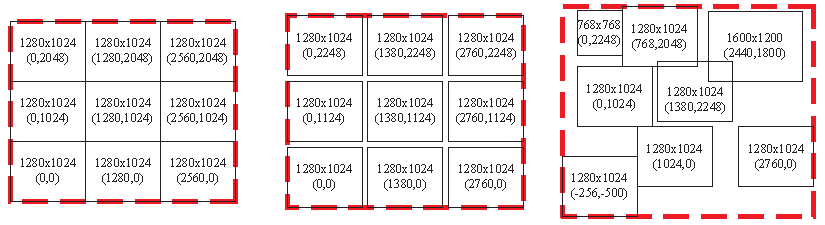
\includegraphics{images/ExampleTileConfig}
  \caption[Defining a tile display.]{Defining a tile display with viewports
    in a logical global display.  Three possible tile arrangements are
    shown.  The bounds of each tile is drawn with the viewport given
    inside.  The viewable area is shown with a dashed line.}
  \label{fig:BasicUsage:tile_layout}
\end{figure}

Figure~\ref{fig:BasicUsage:tile_layout} shows some possible tile
arrangements.  Mullions or overlaps of the tiles in the physical display
can be represented by the spacing or overlap of the viewports in the
logical display.  \IceT does not require the tile layout to have any
regularity.  Chaotic layouts like that shown in the right image of
Figure~\ref{fig:BasicUsage:tile_layout} are legal, although probably not
very useful.  It is allowed, and in fact encouraged, to have processes that
are not directly connected to the tiled display.  These
\index{non-display~process}\keyterm{non-display} processes still contribute
to the image compositing work and will reduce the overall time to render an
image.

The display is defined using the \CFunc{icetResetTiles} and
\CFunc{icetAddTile} functions.  Any previous tile definition is first
cleared out using \CFunc{icetResetTiles} and new tiles are added, one at a
time, using \CFunc{icetAddTile}.

\begin{Table}{3}
  \textC{void }\CFunc{icetResetTiles}\textC{(}&\textC{void}&\textC{)}
\end{Table}

\begin{Table}{3}
  \textC{int }\CFunc{icetAddTile}\textC{(}&\textC{IceTInt}&\CArg{x}\textC{,} \\
    &\textC{IceTInt}&\CArg{y}\textC{,} \\
    &\textC{IceTSizeType}&\CArg{width}\textC{,} \\
    &\textC{IceTSizeType}&\CArg{height}\textC{,} \\
    &\textC{int}&\CArg{display\_rank}\quad\textC{);}
\end{Table}

Each tile is specified using screen coordinates in the logical global
display: the position of the lower left corner and the width and height of
the tile.  Each tile also has a \index{display~process}\keyterm{display
  process} associated with it.  After an image is completely rendered and
composited, the screen section belonging to this tile will be placed in the
process at the given rank.

The following code demonstrates a common example for establishing the tile
layout: a grid of projectors.  The arrangement of projectors in this
example assume that the projectors are connected to processes in the order
of left to right and then top to bottom, which is common.  Note, however,
that \IceT defines its logical global display with $y$ values from the
bottom up like OpenGL does.

\begin{code}
icetResetTiles();
for (row = 0; row < num_tile_rows; row++) {
    for (column = 0; column < num_tile_columns; column++) {
        icetAddTile(column*TILE_WIDTH, (num_tile_rows-row-1)*TILE_HEIGHT,
                    TILE_WIDTH, TILE_HEIGHT,
                    row*num_tile_columns + column);
    }
}
\end{code}

\index{mullion}\keyterm{Mullions} are added by simply spacing the tiles
apart from each other in the logical global display.  Because they are
defined in the logical global display, physical dimensions of the mullions
must first be converted to pixels using the dot pitch of the displays.  The
following code adds mullions between all of the tiles.

\begin{code}
icetResetTiles();
for (row = 0; row < num_tile_rows; row++) {
    for (column = 0; column < num_tile_columns; column++) {
        icetAddTile(column*(TILE_WIDTH + x_mullion),
                    (num_tile_rows-row-1)*(TILE_HEIGHT + y_mullion),
                    TILE_WIDTH, TILE_HEIGHT,
                    row*num_tile_columns + column);
    }
}
\end{code}

An equally common use for \IceT is to render images in parallel to a single
display.  In this \index{single-tile~rendering}\keyterm{single-tile
  rendering} mode, we simply create a single tile whose image will be
placed in the GUI of some application.  This is done by either using the
OpenGL context of the GUI as part of the \IceT rendering process or by
grabbing the image of the single tile and copying into the GUI.  The
example code below sets up \IceT to create a single image that is
accessible on the root process.

\begin{code}
icetResetTiles();
icetAddTile(0, 0, SCREEN_WIDTH, SCREEN_HEIGHT, 0);
\end{code}

\IceT indexes the tiles in the order that they are defined with
\CFunc{icetAddTile}.  You can get the current definition of the tile
display from a number of state variables, which can be retrieved as always
with \CFunc{icetGet}.  \CEnum{ICET\_NUM\_TILES} stores the number of tiles
that are defined (the number of times \CFunc{icetAddTile} was called).
\CEnum{ICET\_TILE\_VIEWPORTS} stores an array with all of the dimensions of
each tile.  For each tile, \CEnum{ICET\_TILE\_VIEWPORTS} contains the four
\index{viewport}values $\langle x, y, width, height \rangle$, stored
consecutively, corresponding to the values passed to \CFunc{icetAddTile}.
\CEnum{ICET\_DISPLAY\_NODES} stores an array giving the rank of the
\index{display~process}display process displaying that tile.  Each process
can also query the \CEnum{ICET\_TILE\_DISPLAYED} variable to see which tile
is displayed locally.  \CEnum{ICET\_TILE\_DISPLAYED} is set to $-1$ on
every process that does not display a tile.

You can get information about the display geometry as a whole through
\CEnum{ICET\_GLOBAL\_VIEWPORT}.  This variable stores the four-tuple
$\langle x, y, width, height \rangle$.  $x$ and $y$ are placed at the
leftmost and lowest position of all the tiles, and $width$ and $height$ are
just big enough for the viewport to cover all tiles.

The \IceT image compositor remains decoupled from the rendering system.
Calling \CFunc{icetAddTile} will not create a display context or renderable
window for the tile.  That responsibility is left to the calling
application.  When using \IceT in \index{single-tile~rendering}single-tile
rendering mode, the rendering system should be set to produce images of
that single tile's size.  When driving a physical tiled display, each
display process must create a window that covers the entire display.  It is
also a good idea to disable the mouse cursor in these windows.

Note that the size of the tiles do not have to match each other.  Also, the
size of the images that your application generates do not have to match the
size of any of the tiles.  There is, however, a constraint that the
generated images on all processes must be at least as large as the largest
tile in each dimension.  To help you maintain that constraint, \IceT stores
the largest tile dimensions in the \CEnum{ICET\_TILE\_MAX\_WIDTH} and
\CEnum{ICET\_TILE\_MAX\_HEIGHT} state variables.

\IceT must know in advanced the size of images that your application will
render.  If you are using \IceT's \OpenGL layer, \IceT will automatically
know the size of the images you generate based off of the current \OpenGL
viewport (retrieved with the \CEnum{GL\_VIEWPORT} \OpenGL state variable).
Otherwise, you can specify the size of images the application generates
with \CFunc{icetPhysicalRenderSize}.  If you are not using the \OpenGL
layer and you have not called \CFunc{icetPhysicalRenderSize}, \IceT assumes
that you will generate images of width \CEnum{ICET\_TILE\_MAX\_WIDTH} and
height \CEnum{ICET\_TILE\_MAX\_HEIGHT}.  The actual expected rendered image
size is stored in the \CEnum{ICET\_PHYSICAL\_RENDER\_WIDTH} and
\CEnum{ICET\_PHYSICAL\_RENDER\_HEIGHT} state variables.

Although counterintuitive, it is often more efficient to create images that
are larger than any tile.  This situation may be necessary when using
\index{image!inflation}image inflation (see
Chapter~\ref{sec:Customizing_Compositing:Image_Inflation}).  Even when not
using image inflation, larger rendered images can save a significant amount
of rendering time.  \IceT can use the larger images to potentially render
in one shot an object that is larger than any of the tiles.

\index{display~definition|)}
\index{tile~definition|)}


\section{Strategies}
\label{sec:Basic_Usage:Strategies}

\index{strategy|(}

\IceT contains several algorithms for performing image compositing.  The
overall algorithm used to render and composite an image is called a
strategy, named after the ``Gang of Four'' strategy pattern.\footnote{Erich
  Gamma, Richard Helm, Ralph Johnson, and John Vlissides.  \emph{Design
    Patterns}.  Addison-Wesley, 1994.  ISBN 0-201-63361-2.}  The strategy
is set using the \CFunc{icetStrategy} function.

\begin{Table}{3}
  \textC{void }\CFunc{icetStrategy}\textC{(}&\textC{IceTEnum}&\CArg{strategy}\quad\textC{);}
\end{Table}

\IceT defines the following strategies that can be passed to
\CFunc{icetStrategy}.  These strategies are discussed in more detail in
Chapter~\ref{chap:Strategies}.

% -*- latex -*-

  \begin{Description}
  \item[\CEnum{ICET\_STRATEGY\_SEQUENTIAL}]
    Basically applies a ``traditional'' single tile composition (such as
    binary swap) to each tile in the order they were defined.  Because each
    process must take part in the composition of each tile regardless of
    whether they draw into it, this strategy is usually inefficient when
    compositing for more than one tile, but is recommended for the single
    tile case because it bypasses some of the communication necessary for
    the other multi-tile strategies.
    \index{strategy!sequential}
  \item[\CEnum{ICET\_STRATEGY\_DIRECT}] As each process renders an image
    for a tile, that image is sent directly to the process that will
    display that tile.  This usually results in a few processes receiving
    and processing the majority of the data, and is therefore usually an
    inefficient strategy.
    \index{strategy!direct}
  \item[\CEnum{ICET\_STRATEGY\_SPLIT}] Like \CEnum{ICET\_STRATEGY\_DIRECT},
    except that the tiles are split up, and each process is assigned a
    piece of a tile in such a way that each process receives and handles
    about the same amount of data.  This strategy is often very efficient,
    but due to the large amount of messages passed, it has not proven to be
    very scalable or robust.
    \index{strategy!split}
  \item[\CEnum{ICET\_STRATEGY\_REDUCE}] A two phase algorithm.  In the
    first phase, tile images are redistributed such that each process has
    one image for one tile.  In the second phase, a ``traditional'' single
    tile composition is performed for each tile.  Since each process
    contains an image for only one tile, all these compositions may happen
    simultaneously.  This is a well rounded strategy that seems to perform
    well in a wide variety of multi-tile applications.  (However, in the
    special case where only one tile is defined, the sequential strategy is
    probably better.)
    \index{strategy!reduce}
  \item[\CEnum{ICET\_STRATEGY\_VTREE}] An extension to the binary tree
    algorithm for image composition.  Sets up a ``virtual'' composition
    tree for each tile image.  Processes that belong to multiple trees
    (because they render to more than one tile) are allowed to float
    between trees.  This strategy is not quite as well load balanced as
    \CEnum{ICET\_STRATEGY\_REDUCE} or \CEnum{ICET\_STRATEGY\_SPLIT}, but
    has very well behaved network communication.
    \index{strategy!virtual~trees}
  \end{Description}


You can get a human-readable name using the \CFunc{icetGetStrategyName}
function.

\begin{Table}{3}
  \textC{const char *}\CFunc{icetGetStrategyName}\textC{(}&\textC{void}&\textC{);}
\end{Table}

The algorithms in \IceT's strategies are specially designed to composite
data defined on multiple tiles.  Some of these algorithms, namely
\CEnum{ICET\_STRATEGY\_REDUCE} and \CEnum{ICET\_STRATEGY\_SEQUENTIAL},
operate at least in part by compositing single images together.  \IceT also
comes with multiple separate strategies for performing this single image
compositing, and this can be selected with the
\CFunc{icetSingleImageStrategy} function.

\begin{Table}{3}
  \textC{void }\CFunc{icetSingleImageStrategy}\textC{(}&\textC{IceTEnum}&\CArg{strategy}\quad\textC{);}
\end{Table}

\IceT defines the following single image strategies that can be passed to
\CFunc{icetSingleImageStrategy}.  These strategies are discussed in more
detail in Chapter~\ref{chap:Strategies}.

% -*- latex -*-

\begin{Description}
\item[\CEnum{ICET\_SINGLE\_IMAGE\_STRATEGY\_AUTOMATIC}] Automatically
  chooses which single image strategy to use based on the number of
  processes participating in the composition.
  \index{single~image~strategy!automatic}
\item[\CEnum{ICET\_SINGLE\_IMAGE\_STRATEGY\_BSWAP}] The classic binary swap
  compositing algorithm.  At each phase of the algorithm, each process
  partners with another, sends half of its image to its partner, and
  receives the opposite half from its partner.  The processes are then
  partitioned into two groups that each have the same image part, and the
  algorithm recurses.
  \index{single~image~strategy!binary~swap}
\item[\CEnum{ICET\_SINGLE\_IMAGE\_STRATEGY\_TREE}] At each phase, each
  process partners with another, and one of the processes sends its entire
  image to the other.  The algorithm recurses with the group of processes
  that received images until only one process has an image.
  \index{single~image~strategy!tree}
\end{Description}


By default \IceT sets the single image strategy to
\CEnum{ICET\_SINGLE\_IMAGE\_STRATEGY\_AUTOMATIC} when a context is created.
This is the single image strategy that will be used if no other is
selected.

You can get a human-readable name using the
\CFunc{icetGetSingleImageStrategyName} function.

\begin{Table}{3}
  \textC{const char *}\CFunc{icetGetSingleImageStrategyName}\textC{(}&\textC{void}&\textC{);}
\end{Table}

\index{strategy|)}


\section{Drawing Callback}
\label{sec:Basic_Usage::Drawing_Callback}

\index{drawing~callback|(}

Most compositing engines will simply take a group of images and combine them
together.  This approach, however, is unreasonable when compositing the
high resolution images on a large tiled display.  It is problematic for an
application to create images larger than any color buffer the rendering
hardware can create, and holding many of these large images can lead to a
large memory profile.

Instead, the \IceT algorithms deal with pieces of the overall image.  The
image pieces are created on demand.  As such, \IceT may require the same
geometry to be rendered multiple times in a single frame.  \IceT provides
the application with the most flexible way to define the rendering process:
with a \keyterm{drawing callback}.

A drawing callback is simply a function that your application provides
\IceT.  When \IceT needs an image, it will provide the drawing callback
with the projection matrices for the section of the display being
rendered.  The drawing callback then returns the image rendered to those
projection matrices.

\IceT may call the drawing callback several times to create a single tiled
image or not at all if the current bounds lie outside the current view
frustum.  This can have a subtle but important impact on the behavior of
the drawing callback.  For example, counting frames by incrementing a frame
counter in the drawing callback is obviously wrong (although you could
count how many times a render occurs).  The drawing callback should also
leave the rendering system in a state such that it will be correct for a
subsequent run of the drawing callback.  Any state that is assumed to be
true on entrance to the drawing callback should also be true on return.

\subsection{Generic Drawing Callback}
\label{sec:Basic_Usage:Drawing_Callback:Generic}

There are two versions of drawing callbacks.  The first version is a
generic callback set with \CFunc{icetDrawCallback}.  This callback is used
in conjunction with the \CFunc{icetDrawFrame} function (described in the
next section).

\begin{Table}{3}
  \multicolumn{3}{l}{
    \textC{typedef void (*}\CType{IceTDrawCallbackType}\textC{)(}
  } \\
  \qquad\qquad\qquad\qquad\qquad\qquad\qquad\qquad
  &\textC{const IceTDouble *}&\CArg{projection\_matrix}\textC{,} \\
  &\textC{const IceTDouble *}&\CArg{modelview\_matrix}\textC{,} \\
  &\textC{const IceTFloat *}&\CArg{background\_color}\textC{,} \\
  &\textC{const IceTInt *}&\CArg{readback\_viewport}\textC{,} \\
  &\CType{IceTImage}&\CArg{result}\quad\textC{)}
\end{Table}

\begin{Table}{3}
  \textC{void }\CFunc{icetDrawCallback}\textC{(}&\CType{IceTDrawCallbackType}&\CArg{callback}\quad\textC{);}
\end{Table}

\CArg{callback} takes two projection matrices: \CArg{projection\_matrix}
and \CArg{modelview\_matrix}.  Each of these arguments is a 16-value array
that represents a $4 \times 4$ transformation of homogeneous coordinates.
The arrays store the matrices in \index{column-major~order}column-major
order.  Thus, if the values in \CArg{projection\_matrix} are $(p[0],
p[1],... p[15])$ and the values in \CArg{modelview\_matrix} are $(m[0],
m[1],... m[15])$, then a vertex in object space is transformed into
normalized screen coordinates by the sequence of operations

\begin{displaymath}
  \left[
    \begin{array}{cccc}
      p[0] & p[4] & p[8] & p[12] \\
      p[1] & p[5] & p[9] & p[13] \\
      p[2] & p[6] & p[10] & p[14] \\
      p[3] & p[7] & p[11] & p[15]
    \end{array}
  \right]
  \left[
    \begin{array}{cccc}
      m[0] & m[4] & m[8] & m[12] \\
      m[1] & m[5] & m[9] & m[13] \\
      m[2] & m[6] & m[10] & m[14] \\
      m[3] & m[7] & m[11] & m[15]
    \end{array}
  \right]
  \left[
    \begin{array}{c}
      v[0] \\ v[1] \\ v[2] \\ v[3]
    \end{array}
  \right]
\end{displaymath}

More explicitly, if you have a point $(x, y, z, 1)$ in object space stored
in a variable \textC{object\_coord}, you could transform that to world
space in the callback with code like this.

\begin{code}
for (row = 0; row < 4; row++) {
    world_coord[row] = 0.0;
    for (i = 0; i < 4; i++) {
        world_coord[row] += modelview_matrix[row + 4*i] * object_coord[i];
    }
}
\end{code}

Likewise, to transform the \textC{world\_coord} to normalized screen
coordinates, you could apply the following code.

\begin{code}
for (row = 0; row < 4; row++) {
    screen_coord[row] = 0.0;
    for (i = 0; i < 4; i++) {
        screen_coord[row] += projection_matrix[row + 4*i] * world_coord[i];
    }
}
\end{code}

If your rendering system has no need to find the world coordinates of
points, you can combine the two matrices by multiplying them together like
this.

\begin{code}
for (row = 0; row < 4; row++) {
    for (column = 0; column < 4; column++) {
        full_matrix[row + 4*column] = 0.0;
        for (i = 0; i < 4; i++) {
            full_matrix[row + 4*column] +=
                projection_matrix[row + 4*i] * modelview_matrix[k + 4*column];
        }
    }
}
\end{code}

Normalized screen coordinates are such that everything projected onto the
image has coordinates in the range $[-1,1]$ (after dividing by the ``w''
homogeneous coordinate).  The x and y coordinates have to be shifted to get
the corresponding pixel location.  The normalized screen coordinates are
projected to span the physical render size (see
\CFunc{icetPhysicalRenderSize}), which may differ from the size of any
particular tile.  Also, if you are outputting depth values, \IceT expects
values in the range $[0,1]$, so you will have to shift those as well.  Here
is a pedantic code segment to do this final transformation.

\begin{code}
icetGetIntegerv(ICET_PHYSICAL_RENDER_WIDTH, &image_width);
icetGetIntegerv(ICET_PHYSICAL_RENDER_HEIGHT, &image_height);
/* Alternatively, you could get the width and height from the image passed */
/* to the callback like this.                                              */
/* image_width = icetImageGetWidth(result);                                */
/* image_height = icetImageGetHeight(result);                              */
pixel_x = (int)(image_width*0.5*(screen_coord[0]/screen_coord[3] + 1.0));
pixel_y = (int)(image_height*0.5*(screen_coord[1]/screen_coord[3] + 1.0));
depth = 0.5*(screen_coord[2]/screen_coord[3] + 1.0);
\end{code}

The drawing callback should initialize its backdrop to the
\CArg{background\_color}, which may be different than the background color
passed to \CFunc{icetDrawFrame}.

The resulting image should be rendered (or copied) into the
\CType{IceTImage}, \CArg{result}, passed to the callback.  The image will
be sized by the physical render width and height and its format will
conform to that set by \CFunc{icetSetColorFormat} and
\CFunc{icetSetDepthFormat}.  You can get the buffers of the image with the
\icetImageGetColor and \icetImageGetDepth functions.  Data written to these
buffers will become part of the image.  \IceT's image functions are
described in more detail in the following section starting on
page~\pageref{sec:Basic_Usage:Image_Objects}.

\IceT will always send the drawing callback an image sized by the physical
render viewport specified by \CFunc{icetPhysicalRenderSize} for
convenience.  However, \IceT often needs only a subset of these pixels.
\IceT tells the drawing callback the pixels it actually uses with the
\CArg{readback\_viewport} parameter.  \CArg{readback\_viewport} contains 4
integers specifying a region of pixels that \IceT will use.  The first two
value specify the lower-left corner of the region and the next two specify
the width and height of the region.

For example, if the \CArg{readback\_viewport} is set to $(10, 15, 100,
75)$, then \IceT will use only the pixels in the square between x values 10
and 109 and y values between 15 and 89 (both inclusive).  All other pixels
in the image will be ignored.  It is not an error to provide values for the
other pixels, but it is a waste of computation.

\subsection{OpenGL Drawing Callback}
\label{sec:Basic_Usage:Drawing_Callback:OpenGL}

If you are rendering with \OpenGL, then you can remove many of the
complexities of defining a callback by using \CFunc{icetGLDrawCallback} in
conjunction with \CFunc{icetGLDrawFrame}.

\textC{typedef void (*} \CType{IceTGLDrawCallbackType}\textC{)( void );}

\begin{Table}{3}
  \textC{void }\CFunc{icetGLDrawCallback}\textC{(}&\CType{IceTGLDrawCallbackType}&\CArg{callback}\quad\textC{);}
\end{Table}

The \OpenGL version of the drawing callback takes no arguments.  It simply
issues the appropriate \OpenGL calls to render the geometry.  \IceT
internally takes care of setting the appropriate transformations and clear
color, and then reads back your data from the buffer specified by
\CFunc{icetGLSetReadBuffer} after the drawing callback returns.

The \OpenGL drawing callback should \emph{not} modify the
\CEnum{GL\_PROJECTION\_MATRIX} as this would cause \IceT to place image
data in the wrong location in the tiled display and improperly cull
geometry.  It is acceptable to add transformations to
\CEnum{GL\_MODELVIEW\_MATRIX}, but the bounding vertices given with
\CFunc{icetBoundingVertices} or \CFunc{icetBoundingBox} (see the following
section) are assumed to already be transformed by any such changes to the
modelview matrix.  Also, \CEnum{GL\_MODELVIEW\_MATRIX} must be restored
before the draw function returns.  Therefore, any changes to
\CEnum{GL\_MODELVIEW\_MATRIX} are to be done with care and should be
surrounded by a pair of glPushMatrix and glPopMatrix functions.

It is also important that the \OpenGL drawing callback \emph{not} attempt
the change the clear color.  In some compositing modes, \IceT needs to
read, modify, and change the background color.  These operations will be
lost if the drawing callback changes the background color, and severe color
blending artifacts may result.

\subsection{Specifying Geometry Bounds}
\label{sec:Basic_Usage:Drawing_Callback:Bounds}

\IceT can nominally call the drawing callback for every tile in the
display.  However, in almost any real application each process has data
that demonstrates some spatial locality that causes it to be projected on a
relatively small section of the display.  To give \IceT the information it
needs to prevent unnecessary renders, the application needs to provide the
bounds of the local geometry.  This is done using either the
\CFunc{icetBoundingVertices} or the \CFunc{icetBoundingBox} function.

\begin{Table}{3}
  \textC{void }\CFunc{icetBoundingVertices}\textC{(}&\textC{IceTInt}&\CArg{size}\textC{,} \\
    &\textC{IceTEnum}&\CArg{type}\textC{,} \\
    &\textC{IceTSizeType}&\CArg{stride}\textC{,} \\
    &\textC{IceTSizeType}&\CArg{count}\textC{,} \\
    &\textC{const IceTVoid *}&\CArg{pointer}\quad\textC{);}
\end{Table}

\begin{Table}{3}
  \textC{void }\icetBoundingBoxd\textC{(}&\textC{IceTDouble}&\CArg{x\_min}\textC{,} \\
    &\textC{IceTDouble}&\CArg{x\_max}\textC{,} \\
    &\textC{IceTDouble}&\CArg{y\_min}\textC{,} \\
    &\textC{IceTDouble}&\CArg{y\_max}\textC{,} \\
    &\textC{IceTDouble}&\CArg{z\_min}\textC{,} \\
    &\textC{IceTDouble}&\CArg{z\_max}\quad\textC{);}
\end{Table}

\begin{Table}{3}
  \textC{void }\icetBoundingBoxf\textC{(}&\textC{IceTFloat}&\CArg{x\_min}\textC{,} \\
    &\textC{IceTFloat}&\CArg{x\_max}\textC{,} \\
    &\textC{IceTFloat}&\CArg{y\_min}\textC{,} \\
    &\textC{IceTFloat}&\CArg{y\_max}\textC{,} \\
    &\textC{IceTFloat}&\CArg{z\_min}\textC{,} \\
    &\textC{IceTFloat}&\CArg{z\_max}\quad\textC{);}
\end{Table}

With the \CFunc{icetBoundingVertices} function, you specify a set of
vertices whose convex hull completely contains the geometry.  The
\CFunc{icetBoundingBox} function is a convenience function that defines the
container as an axis aligned bounding box.

\index{drawing~callback|)}


\section{Rendering}
\label{sec:Basic_Usage:Rendering}

Once you have set up the \IceT state as described in the previous sections
of this chapter, you are ready to perform parallel rendering.  Rendering is
initiated in \IceT by calling one of the draw frame functions.

\subsection{Generic Rendering}
\label{sec:Basic_Usage:Rendering:Generic}

There are two frame drawing functions.  The first version is independent of
the rendering system and is used in conjunction with the callback set with
\CFunc{icetDrawCallback}.  It is performed by calling
\CFunc{icetDrawFrame}.

\begin{Table}{3}
  \CType{IceTImage}\textC{ }\CFunc{icetDrawFrame}\textC{(}
  &\textC{const IceTDouble *}&\CArg{projection\_matrix}\textC{,} \\
  &\textC{const IceTDouble *}&\CArg{modelview\_matrix}\textC{,} \\
  &\textC{const IceTFloat *}&\CArg{background\_color}\quad\textC{);}
\end{Table}

Conceptually, calling \CFunc{icetDrawFrame} is similar to calling the
\index{drawing~callback}drawing callback directly.  The arguments
\CArg{projection\_matrix}, \CArg{modelview\_matrix}, and
\CArg{background\_color} are the same as you would potentially pass the
callback (although \IceT is free to change them).

The \CArg{projection\_matrix} and \CArg{modelview\_matrix} are 16-value
arrays that represent $4 \times 4$ transformations of homogeneous coordinates.
The arrays store the matrices in \index{column-major~order}column-major
order.  Thus, if the values in \CArg{projection\_matrix} are $(p[0],
p[1],... p[15])$ and the values in \CArg{modelview\_matrix} are $(m[0],
m[1],... m[15])$, then a vertex in object space is transformed into
normalized screen coordinates by the sequence of operations

For example, if your modelview matrix used a simple translation to move the
geometry in front of the camera, you would use a matrix like this.

\begin{displaymath}
  \left[
    \begin{array}{cccc}
      1 & 0 & 0 & x \\
      0 & 1 & 0 & y \\
      0 & 0 & 1 & z \\
      0 & 0 & 0 & 1
    \end{array}
  \right]
\end{displaymath}

The code to set the modelview matrix could look like this.

\begin{code}
modelview_matrix[ 0] = 1.0;
modelview_matrix[ 1] = 0.0;
modelview_matrix[ 2] = 0.0;
modelview_matrix[ 3] = 0.0;

modelview_matrix[ 4] = 0.0;
modelview_matrix[ 5] = 1.0;
modelview_matrix[ 6] = 0.0;
modelview_matrix[ 7] = 0.0;

modelview_matrix[ 8] = 0.0;
modelview_matrix[ 9] = 0.0;
modelview_matrix[10] = 1.0;
modelview_matrix[11] = 0.0;

modelview_matrix[12] = x;
modelview_matrix[13] = y;
modelview_matrix[14] = z;
modelview_matrix[15] = 1.0;
\end{code}

As another example, consider setting the projection matrix for the
perspective of a camera sitting at the origin facing down the $-z$ axis.
You could use a transformation matrix like this.

\begin{displaymath}
  \begin{array}{c}
    \left[
      \begin{array}{cccc}
        \frac{f \cdot height}{width} & 0 & 0 & 0 \\
        0 & f & 0 & 0 \\
        0 & 0 & -1 & -2near \\
        0 & 0 & -1 & 0
      \end{array}
    \right] \\
    f = \mathrm{cotangent}\left(\frac{fovy}{2}\right)
  \end{array}
\end{displaymath}

The code to set the projection matrix could look like this.

\begin{code}
/* width, height: image dimensions */
/* fovy: field of view in the y direction */
/* zNear: distance from camera (at origin) to near clipping plane (at -zNear). */

f = 1.0/tan(0.5*fovy);

projection_matrix[ 0] = (f*height)/width;
projection_matrix[ 1] = 0.0;
projection_matrix[ 2] = 0.0;
projection_matrix[ 3] = 0.0;

projection_matrix[ 4] = 0.0;
projection_matrix[ 5] = f;
projection_matrix[ 6] = 0.0;
projection_matrix[ 7] = 0.0;

projection_matrix[ 8] = 0.0;
projection_matrix[ 9] = 0.0;
projection_matrix[10] = -1.0;
projection_matrix[11] = -1.0;

projection_matrix[12] = 0.0;
projection_matrix[13] = 0.0;
projection_matrix[14] = -2*zNear;
projection_matrix[15] = 0.0;
\end{code}

The \CArg{background\_color} is the color in which the background should be
initialized.  It is the color of ``empty'' pixels and also the color to be
blended with any transparent geometry.

\CFunc{icetDrawFrame} returns an \CType{IceTImage} containing the composited
image displayed on this process.  If the process is not displaying a tile,
then the contents of the image is undefined.

\subsection{OpenGL Rendering}
\label{sec:Basic_Usage:Rendering:OpenGL}

If you are rendering with \OpenGL, then you can remove many of the
complexities of defining projection matrices and displaying images by using
the \CFunc{icetGLDrawFrame} function in conjunction with the drawing
callback set with \CFunc{icetGLDrawCallback}.

\begin{Table}{3}
  \textC{void}\quad\CFunc{icetGLDrawFrame}\textC{( void );}
\end{Table}

\CFunc{icetGLDrawFrame} is called in basically the same way as the \OpenGL
\index{drawing~callback}drawing callback would be called directly.  First,
establish the \OpenGL state.  Setting up the \CEnum{GL\_PROJECTION\_MATRIX}
before calling \CFunc{icetGLDrawFrame} is essential.  It is also advisable
to set up whatever transformations in the \CEnum{GL\_MODELVIEW\_MATRIX}
that you can before calling \CFunc{icetGLDrawFrame}.  \IceT will use and
modify these two matrices to render regions of the tiled display.  The
drawing callback should behave as if neither of the matrices were modified.

By the time \CFunc{icetGLDrawFrame} completes, an image will have been
completely rendered and composited.  If \CEnum{ICET\_GL\_DISPLAY} is
enabled, then the fully composited image is written back to the \OpenGL
frame buffer for display.  It is the application's responsibility to
synchronize the processes and swap front and back buffers.  The image
remaining in the frame buffer is undefined if \CEnum{ICET\_GL\_DISPLAY} is
disabled or the process is not displaying a tile.

If the \OpenGL background color is set to something other than black,
\CEnum{ICET\_GL\_DISPLAY\_COLORED\_BACKGROUND} should also be enabled.
Displaying with \CEnum{ICET\_GL\_DISPLAY\_COLORED\_BACKGROUND} disabled may
be slightly faster (depending on graphics hardware) but can result in black
rectangles in the background.

If \CEnum{ICET\_GL\_DISPLAY\_INFLATE} is enabled and the size of the
renderable window (determined by the current \OpenGL viewport) is greater
than that of the tile being displayed, then the image will first be
``inflated'' to the size of the actual display.  If
\CEnum{ICET\_GL\_DISPLAY\_INFLATE} is disabled, the image is drawn at its
original resolution at the lower left corner of the display.  More details
on image inflation are given in
Chapter~\ref{sec:Customizing_Compositing:Image_Inflation}.

Regardless of whether it writes the fully composited image back to the
display, \CFunc{icetGLDrawFrame} returns an \CType{IceTImage} containing
the composited image displayed on this process.  If the process is not
displaying a tile, then the contents of the image is undefined.


\section{Image Objects}
\label{sec:Basic_Usage:Image_Objects}

\IceT uses a data type called \CType{IceTImage} to store and pass around
image data.  To get image data from a generic drawing callback (described
previously starting on
page~\pageref{sec:Basic_Usage:Drawing_Callback:Generic}), \IceT passes the
callback an \CType{IceTImage} sized to hold an image of the appropriate
dimensions.  Likewise, the frame drawing functions (described previously
starting on page~\pageref{sec:Basic_Usage:Rendering}) return an
\CType{IceTImage}.  An \CType{IceTImage} is intended to be an opaque object
that is accessed by a suite of functions provided by \IceT.

\index{null image|see{image, null}}

\IceT defines a special \index{image!null}\keyterm{null image} that can be
used as a place holder when no image data is available.  You can create and
check for null images with the \CFunc{icetImageNull} and
\CFunc{icetImageIsNull} functions, respectively.

\begin{Table}{3}
  \CType{IceTImage}\textC{ }\CFunc{icetImageNull}\textC{(}&\textC{void}&\textC{);}
\end{Table}
\begin{Table}{3}
  \textC{IceTBoolean}\textC{ }\CFunc{icetImageIsNull}\textC{(}&\CType{IceTImage}&\CArg{image}\quad\textC{);}
\end{Table}

It is good defensive programming to initialize \CType{IceTImage} objects to
null on creation.  That way, all of \IceT's images functions will always
behave appropriately on the image, whereas the behavior is unpredictable if
the \CType{IceTImage} is uninitialized.

\begin{code}
IceTImage image = icetImageNull();
\end{code}

The functions \CFunc{icetImageGetWidth}, \CFunc{icetImageGetHeight}, and
\CFunc{icetImageGetNumPixels} return the dimensions of an image.

\begin{Table}{5}
  \textC{IceTSizeType}&\icetImageGetWidth&\textC{(}\quad\textC{const }\CType{IceTImage}&\CArg{image}&\textC{);} \\
  \textC{IceTSizeType}&\icetImageGetHeight&\textC{(}\quad\textC{const }\CType{IceTImage}&\CArg{image}&\textC{);} \\
  \textC{IceTSizeType}&\icetImageGetNumPixels&\textC{(}\quad\textC{const }\CType{IceTImage}&\CArg{image}&\textC{);}
\end{Table}

An \CType{IceTImage} can hold color data, depth data, or both.
Furthermore, colors and depths can be stored in different formats.  The
internal formats for colors and depths for an \CType{IceTImage} can be
retrieved with the \CFunc{icetImageGetColorFormat} and
\CFunc{icetImageGetDepthFormat} functions, respectively.

\begin{Table}{5}
  \textC{IceTEnum}&\icetImageGetColorFormat\textC{(}&\textC{const }\CType{IceTImage}&\CArg{image}&\textC{);} \\
  \textC{IceTEnum}&\icetImageGetDepthFormat\textC{(}&\textC{const }\CType{IceTImage}&\CArg{image}&\textC{);}
\end{Table}

The format specifies the basic data type, the packing, and whether the
color or depth data is available at all.  Here is a list of possible color
formats.

% -*- latex -*-

  \begin{Description}[ICET\_IMAGE\_COLOR\_RGBA\_UBYTE]
  \item[\CEnum{ICET\_IMAGE\_COLOR\_RGBA\_UBYTE}] Each entry is an RGBA
    color tuple.  Each component is valued in the range from $0$ to $255$
    and is stored as an 8-bit integer.  The buffer will always be allocated
    on memory boundaries such that each color value can be treated as a
    single 32-bit integer.
  \item[\CEnum{ICET\_IMAGE\_COLOR\_RGBA\_FLOAT}] Each entry is an RGBA
    color tuple.  Each component is in the range from $0.0$ to $1.0$ and is
    stored as a 32-bit float.
  \item[\CEnum{ICET\_IMAGE\_COLOR\_RGB\_FLOAT}] Each entry is an RGB color
    triple. Each component is in the range from $0.0$ to $1.0$ and is
    stored as a 32-bit float. Note that there is no alpha channel, so the
    color blending composite mode will not work with this color format.
  \item[\CEnum{ICET\_IMAGE\_COLOR\_NONE}] No color values are stored in the
    image.
  \end{Description}



Here is a list of possible depth formats.

% -*- latex -*-

  \begin{Description}[ICET\_IMAGE\_COLOR\_RGBA\_UBYTE]
  \item[\CEnum{ICET\_IMAGE\_DEPTH\_FLOAT}] Each entry is in the range from
    $0.0$ (near plane) to $1.0$ (far plane) and is stored as a 32-bit
    float.
  \item[\CEnum{ICET\_IMAGE\_DEPTH\_NONE}] No depth values are stored in the
    image.
  \end{Description}


An \CType{IceTImage} stores the color and depth data in separate buffers.
You can use the \icetImageGetColor and \icetImageGetDepth functions to
retrieve pointers to this data.  A drawing callback must use these
functions to get buffers to write data into.

\begin{Table}{4}
  \textC{IceTUByte *}&\icetImageGetColorub&\textC{(}\quad\CType{IceTImage}&\CArg{image}\quad\textC{)}; \\
  \textC{IceTUInt *}&\icetImageGetColorui&\textC{(}\quad\CType{IceTImage}&\CArg{image}\quad\textC{)}; \\
  \textC{IceTFloat *}&\icetImageGetColorf&\textC{(}\quad\CType{IceTImage}&\CArg{image}\quad\textC{)}; \\
  \\
  \textC{IceTFloat *}&\icetImageGetDepthf&\textC{(}\quad\CType{IceTImage}&\CArg{image}\quad\textC{)};
\end{Table}

The various forms of \icetImageGetColor and \icetImageGetDepth return typed
arrays for the buffer of data.  The type of the data must conform to the
internal format of the data; the functions will raise an error otherwise.

If you want to use image data of a specific format, you can use one of the
\icetImageCopyColor or \icetImageCopyDepth functions.  With these
functions, you give an allocated array and a specific color format, and the
data for that array will be copied into your buffer in the desired format.

\begin{Table}{4}
  \textC{void}&\icetImageCopyColorub\textC{(}&\textC{const }\CType{IceTImage}&\CArg{image}\textC{,} \\
  &&\textC{IceTUByte *}&\CArg{color\_buffer}, \\
  &&\textC{IceTEnum}&\CArg{color\_format}\quad\textC{);} 
\end{Table}

\begin{Table}{4}
  \textC{void}&\icetImageCopyColorf\textC{(}&\textC{const }\CType{IceTImage}&\CArg{image}\textC{,} \\
  &&\textC{IceTFloat *}&\CArg{color\_buffer}, \\
  &&\textC{IceTEnum}&\CArg{color\_format}\quad\textC{);}
\end{Table}

\begin{Table}{4}
  \textC{void}&\icetImageCopyDepthf\textC{(}&\textC{const }\CType{IceTImage}&\CArg{image}\textC{,} \\
  &&\textC{IceTFloat *}&\CArg{depth\_buffer}, \\
  &&\textC{IceTEnum}&\CArg{depth\_format}\quad\textC{);}
\end{Table}

